\section{Marco teórico}

\subsection{Sonido y resonancia}

El sonido en el aire se propaga como una onda mecánica longitudinal, formada por variaciones de presión y densidad en la dirección de propagación. La frecuencia $f$, medida en hertz (\si{\hertz}), indica el número de oscilaciones por segundo; la amplitud describe la magnitud de la perturbación, mientras que la intensidad sonora corresponde a la potencia acústica transportada por unidad de área y es proporcional al cuadrado de la amplitud de presión para una onda armónica. La velocidad de propagación $v$ (\si{\meter\per\second}), la longitud de onda $\lambda$ (\si{\meter}) y la frecuencia se relacionan mediante \cite{halliday2018,openstax2016}

\begin{equation}
v=\lambda f.
\label{eq:velocidad_onda}
\end{equation}

En un gas, la velocidad del sonido depende de sus propiedades y, en particular, de la temperatura. Para el aire y temperaturas expresadas en grados Celsius, se empleó la aproximación prescrita por la guía de laboratorio \cite{guiauca}

\begin{equation}
v_T=331.25+0.585T,
\label{eq:velocidad_temperatura}
\end{equation}

donde $v_T$ es la velocidad de referencia en \si{\meter\per\second} y $T$ es la temperatura ambiente en \si{\degreeCelsius}. La resonancia acústica ocurre cuando la frecuencia de excitación coincide con una frecuencia natural del sistema, lo que produce una respuesta de amplitud elevada \cite{halliday2018,openstax2016}.

\subsection{Ondas estacionarias en un tubo cerrado}

En un tubo, las ondas sonoras incidentes se superponen con las ondas reflejadas en sus extremos. Para determinadas frecuencias, esta superposición forma ondas estacionarias con posiciones de amplitud fija. En un tubo cerrado por un extremo y abierto por el otro, el desplazamiento del aire presenta un nodo en el extremo cerrado y un antinodo en el extremo abierto; para la presión, estas posiciones se intercambian. Las condiciones de frontera permiten un cuarto de longitud de onda en el modo fundamental y, en el modelo ideal, únicamente los armónicos impares \cite{halliday2018,openstax2016}.

Para expresar las frecuencias permitidas se considera la longitud efectiva $L_f$ del tubo, en metros, que incluye la longitud física $L$ y la corrección de extremo. La longitud de onda del modo $n$ y su frecuencia se escriben como

\begin{equation}
\lambda_n=\frac{4L_f}{n},\qquad n=1,3,5,\ldots,
\label{eq:longitud_onda_tubo}
\end{equation}

\begin{equation}
f_n=\frac{nv}{4L_f}=nf_1,
\label{eq:frecuencias_tubo}
\end{equation}

donde $f_n$ es la frecuencia del modo $n$ en hertz y $f_1$ es la frecuencia fundamental. Para esta última, $n=1$, por lo que

\begin{equation}
f_1=\frac{v}{4L_f}.
\label{eq:fundamental_tubo}
\end{equation}

En contraste, un tubo abierto en ambos extremos presenta antinodos de desplazamiento en los dos extremos y admite, idealmente, todos los armónicos enteros. En un tubo abierto por un extremo, la longitud efectiva excede ligeramente la longitud física debido a que el antinodo se forma fuera de la abertura. Siguiendo la guía, para esta probeta se utiliza la corrección aproximada $0.3D$, donde $D$ es el diámetro interno en metros \cite{guiauca}:

\begin{equation}
L_f=L+0.3D.
\label{eq:correccion_extremo}
\end{equation}

La corrección de extremo aproxima el desplazamiento del antinodo fuera de una abertura libre; su uso depende de la geometría y de la frecuencia. El teléfono puede cubrir parcialmente la boca y alterar esa condición. Por ello, $L_f$ es una longitud acústica efectiva, no la profundidad medida directamente.

\begin{figure}[!t]
\centering
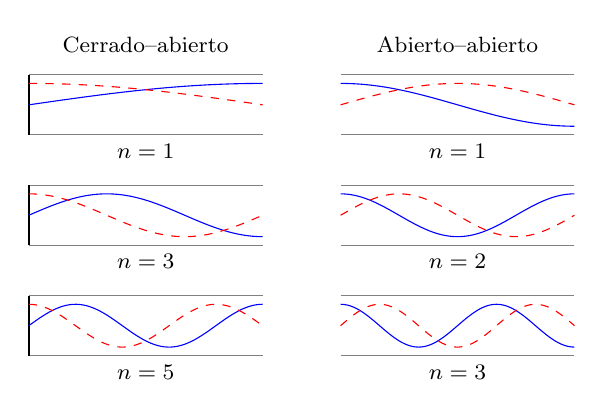
\begin{tikzpicture}[x=1.1cm,y=0.85cm,font=\footnotesize]
\node at (1.35,4.6) {Cerrado--abierto};
\node at (4.95,4.6) {Abierto--abierto};
\foreach \j/\n in {0/1,1/3,2/5}{
 \begin{scope}[shift={(0,3.7-1.65*\j)}]
 \draw[gray] (0,-.45)--(2.7,-.45) (0,.45)--(2.7,.45);
 \draw[thick] (0,-.45)--(0,.45);
 \draw[blue,domain=0:2.7,samples=70] plot (\x,{.32*sin(\n*90*\x/2.7)});
 \draw[red,dashed,domain=0:2.7,samples=70] plot (\x,{.32*cos(\n*90*\x/2.7)});
 \node[below] at (1.35,-.44) {$n=\n$};
 \end{scope}
}
\foreach \j/\n in {0/1,1/2,2/3}{
 \begin{scope}[shift={(3.6,3.7-1.65*\j)}]
 \draw[gray] (0,-.45)--(2.7,-.45) (0,.45)--(2.7,.45);
 \draw[blue,domain=0:2.7,samples=70] plot (\x,{.32*cos(\n*180*\x/2.7)});
 \draw[red,dashed,domain=0:2.7,samples=70] plot (\x,{.32*sin(\n*180*\x/2.7)});
 \node[below] at (1.35,-.44) {$n=\n$};
 \end{scope}
}
\end{tikzpicture}

\caption{Perfiles espaciales normalizados de desplazamiento (línea continua) y presión (discontinua), en un instante representativo. Tubo cerrado--abierto: $n=1,3,5$; abierto--abierto: $n=1,2,3$. Se representan modos ideales, no mediciones.}
\label{fig:modos_tubos}
\end{figure}
La Fig.~\ref{fig:modos_tubos} compara ambos tipos de tubo. En el tubo abierto--abierto la relación es $f_n=nv/(2L_{\mathrm{ef}})$, con $n=1,2,3,\ldots$; en este caso, la longitud efectiva puede incluir correcciones en ambas aberturas \cite{openstax2016}.

\subsection{Variación de la columna de aire mediante agua}

Al agregar agua a la probeta, el volumen ocupado por el líquido reduce la longitud de la columna de aire y modifica su frecuencia fundamental de resonancia. Si la sección transversal del tubo se considera uniforme y circular, su área interna $A$ se calcula a partir del diámetro interno $D$ \cite{guiauca}:

\begin{equation}
A=\frac{\pi D^2}{4}.
\label{eq:area_tubo}
\end{equation}

La longitud geométrica de aire es $\ell=L-V/A$, mientras que la efectiva es $L'=\ell+0.3D$. Para un volumen de agua $V$, expresado en unidades compatibles con $A$, la longitud efectiva restante de la columna de aire $L'$ es

\begin{equation}
L'=L_f-\frac{V}{A}.
\label{eq:longitud_aire_agua}
\end{equation}

Al sustituir esta longitud en el modelo del tubo cerrado, la frecuencia fundamental queda expresada como

\begin{equation}
f=\frac{v}{4L'}.
\label{eq:frecuencia_longitud_aire}
\end{equation}

Por tanto, $f$ es lineal respecto de $1/L'$, con pendiente teórica $v/4$. Despejando el volumen de las Ecs.~\eqref{eq:longitud_aire_agua} y \eqref{eq:frecuencia_longitud_aire}, se obtiene el volumen requerido para alcanzar resonancia con un diapasón de frecuencia conocida $f$:

\begin{equation}
V=\frac{\pi D^2}{4}\left(L_f-\frac{v_T}{4f}\right).
\label{eq:volumen_resonancia}
\end{equation}

En estas expresiones, $D$ y las longitudes se expresan en metros, $A$ en \si{\meter\squared}, $V$ en \si{\meter\cubed}, y $f$ en \si{\hertz}; así, el término $V/A$ tiene unidades de longitud. Para la estimación basada en la temperatura se utiliza $v_T$ en \si{\meter\per\second}, mientras que en el análisis experimental puede utilizarse la velocidad determinada a partir de las frecuencias medidas.

La Ec.~\eqref{eq:volumen_resonancia} corresponde al modo fundamental. Debe cumplirse $0\leq V\leq AL$ y $L'>0$: un resultado fuera de ese intervalo no describe un nivel de agua realizable. Se supone una sección interna aproximadamente uniforme; un fondo curvo, cambios de diámetro o la lectura del menisco pueden limitar $V/A$.

\subsection{Análisis espectral y relación con el experimento}
El micrófono registra una señal temporal. La transformada discreta de Fourier descompone sus muestras en componentes sinusoidales, obteniendo amplitudes por frecuencia; la FFT es un algoritmo eficiente para calcularla. Los máximos del espectro permiten localizar componentes realzadas durante el barrido y asociarlas con resonancias. El espectro también contiene ruido y la respuesta de los transductores, por lo que no todo máximo identifica necesariamente un modo del tubo \cite{smithdft}.



El modelo relaciona las resonancias identificadas en los barridos con los modos permitidos del tubo y permite estimar la frecuencia fundamental mediante el ajuste lineal de $f_n$ respecto de $n$. La velocidad obtenida se puede contrastar con la referencia calculada a partir de la temperatura ambiente. Asimismo, la dependencia lineal de la frecuencia fundamental con $1/L'$ describe el análisis de la columna de aire para distintos niveles de agua, mientras que el volumen estimado con la Ec.~\eqref{eq:volumen_resonancia} proporciona una condición teórica para comprobar la resonancia con diapasones.
